% Options for packages loaded elsewhere
\PassOptionsToPackage{unicode}{hyperref}
\PassOptionsToPackage{hyphens}{url}
%
\documentclass[
]{article}
\usepackage{amsmath,amssymb}
\usepackage{lmodern}
\usepackage{iftex}
\ifPDFTeX
  \usepackage[T1]{fontenc}
  \usepackage[utf8]{inputenc}
  \usepackage{textcomp} % provide euro and other symbols
\else % if luatex or xetex
  \usepackage{unicode-math}
  \defaultfontfeatures{Scale=MatchLowercase}
  \defaultfontfeatures[\rmfamily]{Ligatures=TeX,Scale=1}
\fi
% Use upquote if available, for straight quotes in verbatim environments
\IfFileExists{upquote.sty}{\usepackage{upquote}}{}
\IfFileExists{microtype.sty}{% use microtype if available
  \usepackage[]{microtype}
  \UseMicrotypeSet[protrusion]{basicmath} % disable protrusion for tt fonts
}{}
\makeatletter
\@ifundefined{KOMAClassName}{% if non-KOMA class
  \IfFileExists{parskip.sty}{%
    \usepackage{parskip}
  }{% else
    \setlength{\parindent}{0pt}
    \setlength{\parskip}{6pt plus 2pt minus 1pt}}
}{% if KOMA class
  \KOMAoptions{parskip=half}}
\makeatother
\usepackage{xcolor}
\usepackage[margin=1in]{geometry}
\usepackage{longtable,booktabs,array}
\usepackage{calc} % for calculating minipage widths
% Correct order of tables after \paragraph or \subparagraph
\usepackage{etoolbox}
\makeatletter
\patchcmd\longtable{\par}{\if@noskipsec\mbox{}\fi\par}{}{}
\makeatother
% Allow footnotes in longtable head/foot
\IfFileExists{footnotehyper.sty}{\usepackage{footnotehyper}}{\usepackage{footnote}}
\makesavenoteenv{longtable}
\usepackage{graphicx}
\makeatletter
\def\maxwidth{\ifdim\Gin@nat@width>\linewidth\linewidth\else\Gin@nat@width\fi}
\def\maxheight{\ifdim\Gin@nat@height>\textheight\textheight\else\Gin@nat@height\fi}
\makeatother
% Scale images if necessary, so that they will not overflow the page
% margins by default, and it is still possible to overwrite the defaults
% using explicit options in \includegraphics[width, height, ...]{}
\setkeys{Gin}{width=\maxwidth,height=\maxheight,keepaspectratio}
% Set default figure placement to htbp
\makeatletter
\def\fps@figure{htbp}
\makeatother
\setlength{\emergencystretch}{3em} % prevent overfull lines
\providecommand{\tightlist}{%
  \setlength{\itemsep}{0pt}\setlength{\parskip}{0pt}}
\setcounter{secnumdepth}{5}
\newlength{\cslhangindent}
\setlength{\cslhangindent}{1.5em}
\newlength{\csllabelwidth}
\setlength{\csllabelwidth}{3em}
\newlength{\cslentryspacingunit} % times entry-spacing
\setlength{\cslentryspacingunit}{\parskip}
\newenvironment{CSLReferences}[2] % #1 hanging-ident, #2 entry spacing
 {% don't indent paragraphs
  \setlength{\parindent}{0pt}
  % turn on hanging indent if param 1 is 1
  \ifodd #1
  \let\oldpar\par
  \def\par{\hangindent=\cslhangindent\oldpar}
  \fi
  % set entry spacing
  \setlength{\parskip}{#2\cslentryspacingunit}
 }%
 {}
\usepackage{calc}
\newcommand{\CSLBlock}[1]{#1\hfill\break}
\newcommand{\CSLLeftMargin}[1]{\parbox[t]{\csllabelwidth}{#1}}
\newcommand{\CSLRightInline}[1]{\parbox[t]{\linewidth - \csllabelwidth}{#1}\break}
\newcommand{\CSLIndent}[1]{\hspace{\cslhangindent}#1}
\newcommand{\beginappendix}{ \setcounter{table}{0} \renewcommand{\thetable}{A\arabic{table}} \setcounter{figure}{0} \renewcommand{\thefigure}{A\arabic{figure}} }
\usepackage[capposition=top]{floatrow}
\usepackage{placeins}
\usepackage{setspace}
\usepackage{dcolumn}
\usepackage{booktabs}
\usepackage{siunitx}
\usepackage{amsmath}
\usepackage{enumerate}
\usepackage[shortlabels]{enumitem}
\usepackage[hang,flushmargin]{footmisc}
\usepackage{makecell}
\usepackage{booktabs}
\usepackage{longtable}
\usepackage{array}
\usepackage{multirow}
\usepackage{wrapfig}
\usepackage{float}
\usepackage{colortbl}
\usepackage{pdflscape}
\usepackage{tabu}
\usepackage{threeparttable}
\usepackage{threeparttablex}
\usepackage[normalem]{ulem}
\usepackage{makecell}
\usepackage{xcolor}
\ifLuaTeX
  \usepackage{selnolig}  % disable illegal ligatures
\fi
\IfFileExists{bookmark.sty}{\usepackage{bookmark}}{\usepackage{hyperref}}
\IfFileExists{xurl.sty}{\usepackage{xurl}}{} % add URL line breaks if available
\urlstyle{same} % disable monospaced font for URLs
\hypersetup{
  pdftitle={Air pollution and agricultural productivity in a developing country},
  pdfauthor={Joshua D. Merfeld},
  hidelinks,
  pdfcreator={LaTeX via pandoc}}

\title{Air pollution and agricultural productivity in a developing country\footnote{I thank Ariel Ortiz-Bobea, Marc Bellemare, and David Sungho Park for comments and suggestions that greatly improved the quality of the paper. The usual disclaimer applies. All scripts used in this paper are publicly available on my GitHub page: github.com/JoshMerfeld/pollution\_development}}
\author{Joshua D. Merfeld\footnote{KDI School of Public Policy and Management and IZA; \href{mailto:merfeld@kdis.ac.kr}{\nolinkurl{merfeld@kdis.ac.kr}}}}
\date{2023-04-13}

\begin{document}
\maketitle
\begin{abstract}
\noindent I document externalities in the agricultural sector of India due to air pollution. Using variation in pollution induced by changes in wind, I show that higher levels of particulate matter lead to decreased agricultural productivity, with changes in productivity of 10 percent being common. Combining wind direction with the rollout of coal plants, results indicate pollution from coal plants has a larger effect on agricultural productivity than other types of pollution. Given that the agricultural sector is a refuge for the poor in many developing countries, these results suggest that the effects of pollution may hit the poorest particularly hard.\\
\strut \\
\textbf{\textit{Keywords}}: pollution, productivity, agriculture, labor, India\\
\textbf{\textit{JEL Codes}}: H40, I15, J22, O13, Q52, Q53
\end{abstract}

\newpage
\doublespacing

\hypertarget{introduction}{%
\section{Introduction}\label{introduction}}

While reliance on coal is declining in much of the world, it continues to be an important source of energy in many countries. In 2021, energy generation from coal reached an all-time high,\footnote{www.iea.org/reports/coal-fired-electricity} driven in part by rapid population growth in developing countries, including India. From 1990 to 2010, India's population grew by more than 40 percent, leading to a large increase in demand for power.\footnote{data.worldbank.org} While natural gas has become a popular alternative in much of the world, the Indian government met much of the increased demand through the construction of coal power plants. During those same two decades, power generation from all coal units of at least 30 megawatts in the country more than doubled, from 42.4 gigawatts to more than 100 gigawatts.\footnote{globalenergymonitor.org/}

There are no doubt positive effects from this increase in power generation; for example, electricity may lead to economic and productivity growth (Dinkelman 2011; Kline and Moretti 2014; Rud 2012; Van de Walle et al. 2017), though electrification alone may not be a sufficient condition (K. Lee, Miguel, and Wolfram 2020). These improvements do not come without downsides, however, especially when it comes to power derived from coal. Pollutants from coal contribute to climate change and the phase out of coal energy is therefore a major climate goal (IEA 2022). Emissions from the production and burning of coal are also directly harmful to health and the environment, including pollutants like sulfur dioxide, nitrogen oxides, and mercury, to name but a few.\footnote{www.eia.gov/energyexplained/coal/coal-and-the-environment.php} While the use of coal had been declining, recent events -- including Russia's invasion of Ukraine -- have led to an increase in the demand for coal.\footnote{www.npr.org/2022/08/15/1117560560/a-rising-demand-for-coal-amidst-war-in-ukraine}

In addition to coal, pollution more generally is increasing in much of the world. Carbon dioxide equivalent per capita has almost double over the last 50 years in India, more than doubled in Indonesia, and almost tripled in China.\footnote{\url{https://edgar.jrc.ec.europa.eu}} Of course, much of this increase is due to the development process itself; as countries develop, their economies transform, with more people moving out of agriculture and into manufacturing and services (Herrendorf, Rogerson, and Valentinyi 2014). Despite this development, agriculture remains a key sector in many developing countries, employing a large proportion of the poor (Dercon 2009). This also means agriculture is a key sector when it comes to poverty reduction (Christiaensen, Demery, and Kuhl 2011). Given the large effects of pollution on health and previously documented impacts on agriculture, this raises a important question: do rising pollution levels in developing countries threaten agricultural productivity?

In this paper, I study the effects of pollution on agricultural productivity in India. Previous work has suggested that there may be harmful direct effects of air pollution (Heck et al. 1982; Marshall et al. 1997) and water pollution (Reddy and Behera 2006) on agricultural productivity, including work showing that gold mines -- which release large amounts of pollutants into the surrounding environment -- lead to lower agricultural productivity in Ghana (Aragón and Rud 2016). These effects can work through the well-known effects on human health and productivity, but also directly through land productivity. Black carbon in soot, for example, can directly affect solar radiation reaching plants on the surface (Ramanathan and Carmichael 2008; Burney and Ramanathan 2014). Relative to previous work in economics, this paper tackles pollution more broadly, before turning to a specific source of pollution: coal plants. I show that air pollution leads to lower agricultural productivity in India and that pollution from coal plants is particularly harmful to agriculture.

Identifying the causal effects of pollution is difficult. For starters, the construction of coal plants is likely to be endogenous, though the relationship between construction and economic conditions is not a priori clear. On the one hand, governments may locate new plants in fast-growing areas, while on the other hand, they may decide the exact location of plants based on the political power of local citizens (Kopas et al. 2020). In the case of the data I use here, coal plants are constructed in areas with higher population and higher literacy. In terms of agriculture, higher productivity predicts more coal plants in a given year as well as the construction of a coal plant over the next decade, indicating possible bias when estimating OLS regressions of agricultural productivity on pollution levels.

To identify the effects of air pollution on agricultural productivity, I identify areas of high pollution emission using the location of coal plants. While coal plants may add emissions, I show that they are located in areas with relatively higher levels of pollution, in general. Using these locations as point sources of pollution, I use plausibly exogenous changes in wind direction -- in a similar spirit to Deryugina et al. (2019) -- to measure the effects of pollution on key agricultural outcomes. I first plot the location of coal plants in India by year. Using a village-level shapefile, I identify all villages that are located within 30km of a coal plant at any time during the sample period, which comprises the 2000s to the 2010s, with differences across outcomes depending on data availability. I then calculate the direction from each coal plant to all villages within 30km. I include all areas, regardless of whether the coal plant has opened yet, to allow me to disaggregate the effects of pollution from coal plants with other kinds of pollution later in the paper. Using daily wind data and these spatial variables, I create an identifier separately for every village for whether a given village is located downwind from a coal plant on any given day. I then aggregate this exposure variable based on the desired analysis; for agricultural productivity, for example, I create an exposure variable measuring the total number of exposure days in the five-month agricultural season, focusing only on the monsoon (Kharif) season. More days being located downwind from a high-pollution location leads to substantially higher average concentrations of particulate matter 2.5 (PM 2.5).\footnote{PM 2.5 is defined as particulate matter with a diameter of less than 2.5 micrometers.}

Using wind direction as an instrument for particulate matter, an increase of PM 2.5 by one percent leads to a large decrease in agricultural productivity, at around 0.73 percent. Given within-village changes in exposure, pollution could be responsible for swings of 7-to-14 percent in agricultural productivity across years. The IV estimates indicate that the effect of pollution is more negative than naïve OLS estimates, which is consistent with the evidence on the construction of coal plants; higher levels of pollution are correlated with higher levels of agricultural productivity, a relationship that the IV strategy adjusts downwards. Robustness checks confirm these main results. Randomization inference shows that the estimates are robust to alternative measures of uncertainty, while leads of pollution do not affect current agricultural productivity.

Heterogeneity analysis shows that the negative effects of pollution are larger in villages that experience higher median exposure to pollution and in villages with higher initial yields. Finally, given how many poor farmers rely on rainfall and how weather shocks increase across the globe, I also look at possible multiplicative effects of shocks by interacting the pollution variables with a rainfall variable. Higher exposure along with less rainfall increases the negative effect of either shock individually, meaning these shocks are compounding. Given concerns regarding agricultural productivity and climate change, the rise of pollution in India may be particularly problematic for poor farmers.

I find that these effects are mostly transmitted by reductions in farm labor during narrow windows of the growing season, using labor allocation data from the National Sample Survey (NSS). While there do not appear to be large changes in labor allocation patterns when looking at the season as a whole, there is a clear pattern when we break down exposure to pollution by month: higher levels of pollution at the beginning of the monsoon season (June and July) lead to lower levels of farm labor allocation, but no changes in non-farm labor allocation. This matches up well with a similar exercise with agricultural yields: pollution in June is the only month in which there is a negative effect of pollution on agricultural yield. In tandem, these two results point to effects on labor as one mechanism driving the total effects, though I cannot rule out direct effects of pollution on land productivity with my data.

The final set of analyses tries to disentangle the effects of pollution from the effects of coal pollution, specifically, by using wind direction and the rollout of coal plants across the country. Combining instrumental variables with a differences-in-differences strategy, I show that agricultural productivity has an elasticity of around -0.15 with respect to non-coal pollution. The opening of a coal plant, however, triples the elasticity, to more than -0.45, indicating that coal plant emissions are particularly harmful to agricultural productivity, at least in India. This is consistent with coal emissions being quite different from other forms of pollution; for example, coal emissions contain much more mercury than other forms of pollution.

This paper contributes to several strands of literature. First, we already have evidence of effects of pollution on different forms of labor activity. For example, general levels of pollution decrease productivity of call center works in China (Chang et al. 2019), lead people to perform worse on cognitive functions (Ebenstein, Lavy, and Roth 2016; Wen and Burke 2022), and also lead to lower levels of farm labor productivity in California, driven by changes in ozone concentration (Graff Zivin and Neidell 2012). Also in China, He, Liu, and Salvo (2019) find small but significant negative effects of pollution on manufacturing productivity, while Chen, Oliva, and Zhang (2022) show pollution leads to labor out migration. Perhaps relevant to my labor allocation results, Hanna and Oliva (2015) show that decreases in pollution lead to increases in labor allocation, while I show the same relationship in at least a subset of months of the agricultural season. Several papers are closely related to this one. Aragón and Rud (2016) show that gold mines in Ghana have substantial negative impacts on agricultural productivity in the surrounding areas. Burney and Ramanathan (2014) model the effects of climate change and pollutants on agricultural productivity in India. Finally, Sanders and Barreca (2022) actually find that coal emissions can be good for agriculture in the United States, due to the presence of sulfur, which can increase agricultural productivity. This paper differs in three important ways. First, I explore effects of pollution more generally as well as from coal plants, which are much more ubiquitous than gold mines across the world. Second, I use a different identification strategy from either paper, relying on wind blowing pollution from coal plants. Finally, agriculture in India and the United States can be quite different, with the latter being much more mechanized. This means effects of pollution could differ substantially.

I also contribute to the more general literature on the effects of pollution on health. Pollution has substantial negative effects on health in both developing and developed countries (Arceo, Hanna, and Oliva 2016) and we have known of these negative effects for many years (Brunekreef and Holgate 2002; Kampa and Castanas 2008; Pope III and Dockery 2006). Currie et al. (2014) review the literature on the health effects of pollution during adolescence; we have robust evidence of pollution exposure leading to increases in infant mortality, including in developing countries (Heft-Neal et al. 2018, 2019). Since these effects are often driven by heart and lung disease and asthma (Kampa and Castanas 2008), this my explain the labor allocation effects I identify in this paper.

The rest of the paper is organized as follows. I first discuss data and then methodology, in two separate sections. The methodology section discusses the empirical strategy and validates the wind direction variable using data on particulate matter. I present the main results in \autoref{results} before concluding in \autoref{conclusion}.

\hypertarget{data}{%
\section{Data}\label{data}}

\label{data}

The main goal of this paper is to examine whether exposure to pollution and emissions from coal plants, in particular, affect agricultural productivity. I use several sources of data, which I describe here and list in Table \ref{tab:data} of the appendix.

The first set of data lists the location of coal plant across the globe. This data comes from Global Energy Monitor\footnote{globalenergymonitor.org/projects/global-coal-plant-tracker/} and lists all units generating at least 30 megawatts of electricity. The data on coal plants includes the year of opening (and, if applicable, the year of retirement), the GPS (latitude/longitude) location of each plant, and the amount of power produced by the units at each plant. For this paper, I do not use the information on the capacity of the plant.

Figure \ref{fig:plants} in the appendix displays the location of coal plants in India for two specific years: 1990 and 2010. There is a clear increase in the prevalence of coal plants across the country over the two decades. Additionally, the overall capacity from coal plants increased from 42.4 gigawatts to 100.4 gigawatts, an increase of 136.6 percent in just 20 years. This increase is driven both by the roll out of new plants as well as the construction of new units at existing plants, the latter of which is not shown in Figure \ref{fig:plants}.

The second dataset includes agricultural productivity for both the monsoon and winter seasons, from 2002 to 2018. To match other data, I only use the data up to 2013. This data comes from Gangopadhyay et al. (2022) and estimates land productivity (i.e.~yield, in tons per hectare) for the major crops in India, using satellite-derived data. While there is a wealth of literature on measurement error in land (Desiere and Jolliffe 2018; Abay et al. 2022), the authors use a static cropland mask for the productivity estimates. This means that any measurement error will be constant across time and subsumed by the village fixed effects. While the measure of output is also noisy, the use of satellite-derived data and a static cropland mask reduces concerns about measurement error being responsible for the results below, especially since common sources of measurement error are unlikely to be correlated with wind direction. The authors define the monsoon season as June to October and the winter season as November to March. I focus on only the monsoon season and keep the authors' definition when matching across data below. This data is also publicly available from Nature's data-sharing website.\footnote{springernature.figshare.com} Since the main regressions below use village fixed effects, any differences in cropping patterns across areas should not bias estimates on changes, as long as these patterns do not change markedly in response to pollution.

The agricultural productivity data is available as raster files with a resolution of 500m. To aggregate this data up to a useful administrative unit, I use village-level shapefiles provided by Asher et al. (2021) and publicly available on the SHRUG platform.\footnote{www.devdatalab.org/shrug\_download/} I aggregate the agricultural productivity data to the village level by extracting mean productivity for each feature in the shapefile. I do this separately for the monsoon season each year, from 2002 to 2013.

To measure exposure to pollution from coal plants, I first locate all village centroids located within 30km from a coal plant in a given year. I choose 30km due to previous research on the effects of (air) pollution (Aragón and Rud 2016; Bencko and Symon 1977; Li and Gibson 2014). I then calculate the direction from coal plants to all village centroids within that 30km radius. To define exposure, I then pull daily wind direction data from the National Center for Atmospheric Research.\footnote{climatedataguide.ucar.edu/} For each day, I document whether the wind is blowing towards each village centroid\footnote{I define ``towards'' as within five degrees to help take into account that I am using village centroids, using the x and y components of wind speed to calculate angles.} and then temporally aggregate this daily data depending on the temporal definition of the corresponding outcome. For example, agricultural productivity is defined across five months (e.g.~the monsoon season is from June to October) so I count the total days a given village is exposed to wind blowing from \emph{any} coal plant within 30km during those five months.

The top panel in Figure \ref{fig:windexample} in the appendix is an example wind direction raster. The raster shows wind direction for the entirety of India on January 1st, 2010, as well as the location of coal power plants on that date. The prevailing winds on the date differ across the country and, though not shown in the figure, across days. This means that the overall exposure for a given area to coal plant emissions changes across time. I also pull data on particulate matter to help validate this proxy for exposure. This data comes from Hammer et al. (2020) and I also aggregate this to the village using the same method detailed above.

To help understand some of the mechanisms driving the relationship between exposure to emissions and agricultural productivity, I also include household survey data. Unfortunately, I am not aware of any publicly available survey data that covers multiple years and has identifiers below the district level. For example, the ARIS-REDS data\footnote{www.ncaer.org/project/additional-rural-incomes-survey-aris-rural-economic-demographic-survey-reds} includes GPS identifiers for one year, but that only allows GPS matching for a total of two years: 1999 and 2007/2008. The DHS, on the other hand, only has state-level identifiers (except for the newest two waves) and is also not a labor survey. Instead, I use the National Sample Survey (NSS) from the Ministry of Statistics and Programme Implementation.

The NSS is a nationally representative survey that was conducted every couple of years until relatively recently. Many rounds of the NSS also included a module on employment that asked about labor allocation over the previous seven days. I use the 61st, 62nd, 64th, 66th, and 68th rounds of the NSS, all of which include the employment module. The publicly available data also includes the date of survey, which allows me to match pollution exposure to the exact day of the survey.

The biggest issue with using the NSS is that it includes only district-level identifiers. The main exposure variables, on the other hand, are defined at a lower level of aggregation, at the village. I choose to aggregate this village-level exposure to the district level as shown in the second panel of Figure \ref{fig:windexample} -- the district is a randomly selected district in the data, Guna district in Madhya Pradesh. I use the area overlap of the villages with the district to define a weighted average of exposure for the district at a given time. I calculate the area of overlap for each village and the district as well as the overall area of the district and use these variables to define weights for individual villages. Any part of the district that does not overlap with one of the villages -- the white area in Figure \ref{fig:windexample} -- does not have any exposure and, as such, receives a value of zero for exposure.

\hypertarget{methods}{%
\section{Methods}\label{methods}}

\label{identification}

I am primarily interested in the effects of pollution on agricultural productivity. We might consider a regression of the following form:
\begin{gather} y_{it} = \alpha_{i} + \gamma_{t} + \beta PM_{it} + \delta rain_{it} + \psi temp_{it} + \varepsilon_{it}, \end{gather}

where \(y_{it}\) is outcome \(y\) for unit \(i\) at time \(t\), \(\alpha\) is a geographic fixed effects, \(\gamma_t\) is time fixed effects, \(PM_{it}\) is the (log) concentration of particulate matter 2.5, \(rain_{it}\) is total rainfall during the season, and \(temp_{it}\) is average temperature during the season.

However, even with the fixed effects, this regression likely suffers from endogeneity; places with more pollution may be very different from places with less pollution. It is difficult to sign the direction of the bias a priori, because it depends on how the coal plants are placed. For example, if coal plants are placed in places in need of power -- for example, due to rapid growth -- then the estimates might be upwards biased. On the other hand, if officials purposefully place coal plants in poorer areas for political reasons, then the estimates might be downwards biased.

So what are the characteristics of areas near the construction of new coal plants? Table \ref{tab:plantresultstable} presents four separate regressions, using state-level fixed effects due to the spatial variation in coal plants. The first two columns use 1991 census data -- downloaded from SHRUG -- and the second two columns use 2001 census data, all at the village level. The first column presents results from regressing a dummy for whether there is a coal plant within 30km in 1991 on several census variables. Villages with higher populations and higher literacy in 1991 are more likely to be near a coal plant at the time.

\begin{table}

\caption{\label{tab:plantresultstable}Local characteristics and the construction of coal plants}
\centering
\begin{threeparttable}
\begin{tabular}[t]{>{\raggedright\arraybackslash}p{3cm}>{\centering\arraybackslash}p{2cm}>{\centering\arraybackslash}p{2cm}>{\centering\arraybackslash}p{2cm}>{\centering\arraybackslash}p{2cm}}
\toprule
\multicolumn{1}{c}{ } & \multicolumn{2}{c}{1991 census} & \multicolumn{2}{c}{2001 census} \\
\cmidrule(l{3pt}r{3pt}){2-3} \cmidrule(l{3pt}r{3pt}){4-5}
  & 1991 & 2001 & 2001 & 2011\\
\midrule
Population (log) & 0.009 & 0.007* & 0.013* & 0.005\\
 & (0.006) & (0.004) & (0.006) & (0.004)\\
Area (log) & -0.007* & -0.004 & -0.007* & -0.004\\
 & (0.004) & (0.005) & (0.004) & (0.003)\\
Literacy (prop) & 0.080** & 0.037 & 0.073* & 0.036\\
 & (0.029) & (0.028) & (0.039) & (0.026)\\
Ag. productivity &  &  & 0.014** & 0.028***\\
 &  &  & (0.005) & (0.009)\\
Pollution &  &  & 0.047 & 0.014\\
(log PM 2.5) &  &  & (0.045) & (0.018)\\
Sub-sample & all & no plant & all & no plant\\
\midrule
Observations & 283,021 & 264,265 & 508,784 & 469,004\\
\bottomrule
\end{tabular}
\begin{tablenotes}[para]
\item Note: State fixed effects are included in regressions. Standard errors are in parentheses and clustered at the state level. The outcome in the first column is whether the village is within 30km of a coal plant in 1991. The second column is whether a village in 1991 will have a coal plant in 2001, conditional on not having one in 1991. The last two columns are similarly defined, except using 2001 and 2011 as the years. * p<0.10 ** p<0.05 *** p<0.01
\end{tablenotes}
\end{threeparttable}
\end{table}

The second column keeps the 1991 census data but changes the outcome variable to a dummy for whether there \emph{will be} a coal plant constructed within 30km before 2001. This column restricts the sample to only villages that do not already have a coal plant within 30km in 1991. Population and literacy both remain strong predictors of the building of a new coal plant.

The last two columns are particularly relevant to the current results. They present similar results to those in the first two columns, but use the 2001 census data and a dummy for the presence of a coal plant in 2001 and 2011 in columns three and four, respectively. Importantly, I include agricultural productivity in the monsoon season of 2002 -- the earliest year available -- as well as average pollution during the monsoon season for 1998 through 2000 as additional predictors. In 2001, agricultural productivity is a strong predictor for the presence of a coal plant. Moreover, it is also a significant predictor of the construction of a coal plant between 2001 and 2011 (column four). Given that the coefficient is positive, this indicates that coal plants are more likely to be built in areas with higher agricultural productivity. In other words, any selection in the overall location of coal plants would bias against finding negative effects of pollution on agricultural productivity. However, note that this is not the same as looking at wind direction, though comparing the OLS and IV results below leads to the same conclusion regarding selection. Pollution, on the other hand, is not significant but is positive in both columns (and is also logged, just like productivity).

Given the likely endogeneity, I instead turn to a plausibly exogenous source of variation in pollution: wind direction. While the location of a coal plant might be endogenous, the amount of pollution received by a specific village in a given year can vary randomly based on wind direction. By counting the number of days in a given year that a village is downwind from a polluted area and conditioning on village fixed effects and weather (rainfall and temperature), variation across years is plausibly exogenous.

Consider the reduced form effect of wind exposure on agricultural productivity:
\begin{gather} y_{it} = \alpha_{i} + \gamma_{t} + \beta wind_{it} + \delta rain_{it} + \psi temp_{it} + \varepsilon_{it}, \end{gather}

where variables are defined identically to above but with wind as the primary variable of interest instead of pollution. Combining these into a two-stage procedure, we can instrument for pollution using wind direction; small changes in wind direction can lead to large changes in pollution exposure for villages located near point sources of pollution, allowing me to identify the causal effects of pollution by isolating the random component driven by wind direction. This is similar in spirit to Deryugina et al. (2019).

Identification relies on changes in wind direction across time for the same geographic units. In other words, conditional on the fixed effects and weather, I assume changes in wind direction are as good as random and uncorrelated with the outcome -- primarily agricultural productivity in this paper -- except through exposure to pollution.

The inclusion of rainfall and temperature is meant to reduce concerns that wind direction may not affect agricultural productivity but, instead, be correlated with it through changes in weather. For example, prevailing winds from one direction may be associated with dry weather, while winds from another direction may be more likely to carry moisture and rain. It is not a priori clear how this would bias the estimates with respect to pollution and coal plants, however. The differences in weather patterns is very context specific and can differ even for villages located near one another. Nonetheless, adding rainfall and temperature should alleviate some of these concerns.

It is worth taking the time to validate the use of wind direction as a measure of exposure to pollution. Consider the data used for the regressions presented in Table \ref{tab:pollutiontable} of the appendix. The outcome variable is particulate matter -- specifically, \(\mathrm{PM 2.5}\), which is particulate matter no larger than 2.5 micrometers in diameter -- which comes from Hammer et al. (2020). \(\mathrm{PM 2.5}\) is one of the harmful byproducts from coal plants, along with sulfur dioxide, different types of nitrogen oxides, and mercury.\footnote{www.epa.gov/airmarkets/power-plants-and-neighboring-communities} This data is available at the monthly level, so in Table \ref{tab:pollutiontable}, I aggregate wind exposure to the monthly level, as well.

Both the particulate matter data and the wind data is at the village level, which means the regressions in Table \ref{tab:pollutiontable} are at the village level. As such, the geographic fixed effects are village fixed effects and the temporal fixed effects are month fixed effects. Since the exposure variable is at the village level and we follow villages over time, the standard errors are also clustered at the village level. In columns two and four, I switch the month fixed effects for district-month fixed effects, which considers only villages in the same district in the same month.

In addition to serving as an example, Table \ref{tab:pollutiontable} also helps validate the use of wind direction as a proxy for exposure to pollution. The first two columns include all available years of data while the last two columns restrict estimation only to the years for which the agricultural productivity regressions are estimated. Across all four columns, the story is the same: when the wind is blowing in the direction of a village from a coal plant within 30 kilometers, estimated \(\mathrm{PM 2.5}\) is substantially higher.

To put context behind pollution numbers, the World Health Organization's updated guidelines are that average annual exposure should not exceed 15 \(\mathrm{\mu g/m^3}\). For the month, an increase at the midpoint of the estimated range is equal to an increase of 0.2 percent of the maximum recommended mean concentration from the WHO. This is just a single day of wind in the direction of a village. Since this includes all villages located within 30km of a coal plant, this is evidence that wind direction can have serious repercussions on the health of hundreds of millions of people in India.

\hypertarget{identifying-effects-of-pollution-from-coal-plants}{%
\subsection{Identifying effects of pollution from coal plants}\label{identifying-effects-of-pollution-from-coal-plants}}

I use the location of coal plants to identify locations of high pollution, but there can be other pollution sources located near coal plants, as well. I nonetheless want to identify the effects of pollution coming specifically from coal plants. I do this by combining the two-stage procedure above with a differences-in-differences framework. Specifically, I create a new variable identifying the exact year the coal plant opens in a given area and calculate the change in the effects of pollution on agricultural productivity.

Consider the following regression of interest:
\begin{gather} 
y_{it} = \alpha_{i} + \gamma_{t} + \omega PM_{it} + \phi open_{it} + \beta PM_{it}\times open_{it} + \delta rain_{it} + \psi temp_{it} + \varepsilon_{it},
\end{gather}

where the interaction term \(PM_{it}\times open_{it}\) indicates the change in the effect of pollution following the opening of the coal plant. Note that this is not the same as saying that pollution increased; instead, it is focusing on the change in the effect of a change in pollution of one unit on the outcome of interest, agricultural yield. I instrument for both \(PM_{it}\) and \(PM_{it}\times open_{it}\) using wind and the interaction between wind and the open indicator, or \(wind_{it}\times open_{it}\).

\hypertarget{results}{%
\section{Results}\label{results}}

\label{results}

I first present the reduced form results for agricultural productivity. The outcome of all the regressions in this section is the log of agricultural land productivity, which is defined as tons per hectare. The first set of results are in Table \ref{tab:yieldtable}. The unit of analysis is the village-year -- from 2002 to 2013 -- focusing only on the monsoon (kharif) season. The data used to construct the yield measure is calculated using five months of data, so the wind variable is defined for the same five months and is the sum of days in which the wind is pointed towards the village centroid from a coal plant.

The first column presents the most simple results, with only the wind exposure variable and the fixed effects. The second column adds a rainfall and average temperature variable, while the third column includes higher-order weather variables, as well. While the coefficient decreases slightly in magnitude as we move from the first to the second column and the second to the third column, the decrease is relatively small. There is a consistent, negative effect of wind exposure on agricultural productivity.

\begin{table}

\caption{\label{tab:yieldtable}Wind direction and agricultural productivity}
\centering
\begin{threeparttable}
\begin{tabular}[t]{>{\raggedright\arraybackslash}p{4cm}>{\centering\arraybackslash}p{2.5cm}>{\centering\arraybackslash}p{2.5cm}>{\centering\arraybackslash}p{2.5cm}}
\toprule
  & (1) & (2) & (3)\\
\midrule
Wind days & -0.0078*** & -0.0069*** & -0.0062***\\
 & (0.0007) & (0.0007) & (0.0006)\\
Rain (z) &  & 0.0854*** & -0.0424***\\
 &  & (0.0018) & (0.0046)\\
Mean temperature (10s) &  & -0.0021*** & 0.1321***\\
 &  & (0.0001) & (0.0034)\\
Rain squared &  &  & -0.0010***\\
 &  &  & (0.0001)\\
Temperature squared &  &  & -0.0002***\\
 &  &  & \vphantom{1} (0.0000)\\
Rain times Temperature &  &  & 0.0003***\\
 &  &  & (0.0000)\\
\textbf{Fixed effects:} & \textbf{} & \textbf{} & \textbf{}\\
Village & Yes & Yes & Yes\\
Year & Yes & Yes & Yes\\
\midrule
Observations & 1,266,922 & 1,266,922 & 1,266,922\\
\bottomrule
\end{tabular}
\begin{tablenotes}[para]
\item Note: Standard errors are in parentheses and are clustered at the village level. The outcome in all regressions is estimated agricultural yield, defined as tons per hectare. * p<0.10 ** p<0.05 *** p<0.01
\end{tablenotes}
\end{threeparttable}
\end{table}

To put the size of the coefficient in context, it is worth digging a little deeper into the exposure variable. The mean within-village absolute deviation in wind exposure is approximately 2.42 days, meaning that the average change in agricultural productivity from year-to-year due to nothing but changes in wind patterns carrying particulate matter is around 1.5 percent relative to the mean. This implies that swings in agricultural productivity -- due to wind direction -- of several percent are probably quite common, since the absolute deviation includes deviations below and above the mean.

\begin{table}

\caption{\label{tab:yieldtablepm}Particulate matter (PM 2.5) and agricultural productivity}
\centering
\begin{threeparttable}
\begin{tabular}[t]{>{\raggedright\arraybackslash}p{4cm}>{\centering\arraybackslash}p{2.5cm}>{\centering\arraybackslash}p{2.5cm}>{\centering\arraybackslash}p{2.5cm}}
\toprule
  & (1) & (2) & (3)\\
\midrule
Particulate matter & -0.042*** & -0.044*** & -0.032***\\
(log PM 2.5) & (0.003) & (0.003) & (0.003)\\
Weather & No & Yes & Yes\\
Weather (expanded) & No & No & Yes\\
\textbf{Fixed effects:} & \textbf{} & \textbf{} & \textbf{}\\
Village & Yes & Yes & Yes\\
Year & Yes & Yes & Yes\\
\midrule
Observations & 1,266,922 & 1,266,922 & 1,266,922\\
\bottomrule
\end{tabular}
\begin{tablenotes}[para]
\item Note: Standard errors are in parentheses and are clustered at the village level. The outcome in all regressions is estimated agricultural yield, defined as tons per hectare. * p<0.10 ** p<0.05 *** p<0.01
\end{tablenotes}
\end{threeparttable}
\end{table}

Of course, it is not wind, per se, that we are interested in. Instead, we are actually interested in better understanding the effects of exposure to pollution on agricultural productivity. Table \ref{tab:yieldtablepm} presents the same regressions as Table \ref{tab:yieldtable}, with a key difference: instead of wind exposure, it uses log average concentration of \(\mathrm{PM 2.5}\) -- from Hammer et al. (2020) -- during the season as the key explanatory variable. There is again a consistent, negative relationship between particulate matter and agricultural productivity. Since both variables are logged, the coefficients are similar to elasticities, indicating that a one-percent increase in pollution leads to a 0.03-to-0.04 percent decrease in agricultural productivity.

Recall, however, the results from above: coal plants were placed in places with higher average agricultural productivity. This means that the simple regressions in Table \ref{tab:yieldtablepm} might actually be biased upwards: although pollution might negatively affect productivity, pollution is higher in more productive areas due to the endogenous placement of coal plants in the study areas. To recover the actual effect of pollution, we need an instrument. If, conditional on the fixed effects and weather variables, wind direction is exogenous and only affects agricultural productivity through pollution, then it is a valid instrument for pollution.

I present the IV results in Table \ref{tab:yieldtabletwo}, with the first-stage F-statistic at the bottom. The first-stage results make clear how strong of an instrument wind is; all three F-statistics are above 1,000, meeting even the higher bar for the first-stage F-test argued for by D. Lee et al. (2022). Also note that the coefficients are quite different from those in Table \ref{tab:pollutiontable} because the unit of analysis in Table \ref{tab:yieldtabletwo} is the season, while in Table \ref{tab:pollutiontable} the unit of analysis is the month.

The second-stage results first indicate that \(\mathrm{PM 2.5}\) is a very strong predictor of agricultural productivity. Using the results in column three, a one percent increase in particulate matter leads to a 0.73 percent decrease in agricultural productivity. To put this in further perspective, the mean particulate matter concentration is just short of 40 (39.68) in the monsoon sample, while the within-village absolute deviation in particulate matter is 3.98, meaning year-to-year swings of 7-to-14 percent in agricultural productivity due to pollution exposure are common.

The comparison of the results to those in the previous table also confirm the concerns around endogenous placement of coal plants. The coefficients in Table \ref{tab:yieldtabletwo} are always more negative than those in Table \ref{tab:yieldtablepm}, and sometimes substantially so. In other words, the simple regression of agricultural productivity on pollution results in coefficients on pollution that are upwards biased, since higher levels of pollution occur in more productive areas, on average. The IV strategy corrects this bias and leads to a robust, negative relationship between pollution and agricultural productivity.

\begin{table}

\caption{\label{tab:yieldtabletwo}Pollution and agricultural productivity, IV estimates}
\centering
\begin{threeparttable}
\begin{tabular}[t]{>{\raggedright\arraybackslash}p{4cm}>{\centering\arraybackslash}p{2cm}>{\centering\arraybackslash}p{2cm}>{\centering\arraybackslash}p{2cm}}
\toprule
  & (1) & (2) & (3)\\
\midrule
Particulate matter & -0.941*** & -0.813*** & -0.728***\\
(log PM 2.5) & (0.078) & (0.076) & (0.075)\\
Weather & No & Yes & Yes\\
Weather (expanded) & No & No & Yes\\
\textbf{Fixed effects:} & \textbf{} & \textbf{} & \textbf{}\\
Village & Yes & Yes & Yes\\
Year & Yes & Yes & Yes\\
\midrule
F (first stage) & 1,236 & 1,263 & 1,264\\
Observations & 1,266,922 & 1,266,922 & 1,266,922\\
\bottomrule
\end{tabular}
\begin{tablenotes}[para]
\item Note: Standard errors are in parentheses and are clustered at the village level. The outcome in all regressions is estimated agricultural yield, defined as tons per hectare. * p<0.10 ** p<0.05 *** p<0.01
\end{tablenotes}
\end{threeparttable}
\end{table}

\begin{figure}
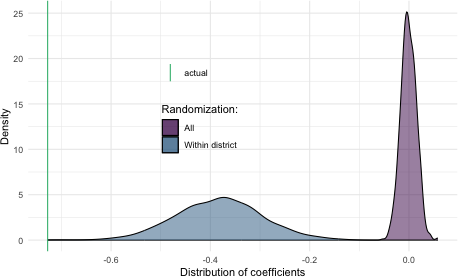
\includegraphics{draft_files/figure-latex/randomplot-1} \caption[Randomization inference]{Randomization inference}\label{fig:randomplot}\floatfoot*{Note: The figure presents the distribution of coefficients by randomly assigning wind direction across villages within the same year. The "all" distribution is created by randomly assigning a single wind value to each village, sampled with replacement across all villages in a given year. The "within district" randomly samples with replacement only from within the same district in the same year.}
\end{figure}

\hypertarget{robustness-checks}{%
\subsection{Robustness checks}\label{robustness-checks}}

In this section, I report the results of two separate robustness checks for the main results presented above. In the previous results, standard errors are clustered at the level of the village, which is also the level at which treatment (exposure to pollution) is assigned as well as the level at which agricultural productivity is extracted. Past work has shown that standard errors might be underestimated in such contexts (Bertrand, Duflo, and Mullainathan 2004). This is a particular concern in the present case, since agricultural productivity is extracted at the village level but estimated using less coarse data that has high spatial correlation (Gangopadhyay et al. 2022).

To help remedy concerns, I perform randomization inference (e.g. Barrios et al. (2012)) by randomly assigning observed treatment across villages and repeating this process 1,000 times. I do this in two separate ways. First, I take all villages in a given year and randomly assign, with replacement, treatment intensity within the year. Second, I do this separately by selecting from within district-years only, to help take into account district-year correlation in outcomes and as a way to mitigate possible concerns that traditional clustered standard errors may actually be much too conservative (Abadie et al. 2023). Since this is an instrumental variables procedure, I randomly select the wind and pollution variable \emph{together}.

I present these results in Figure \ref{fig:randomplot}. The purple density is the resulting distribution of estimated treatment effects when selecting from all villages within the same year. The density of treatment effects is relatively tight around 0, with the left tail only getting slightly beyond -0.05, compared to the most conservative actual estimated treatment effect of -0.73.

The within-district correlation in outcomes and treatment is apparent when instead randomly selecting from only villages within the same district in the same year. The distribution is still approximately normal but has a mode of almost -0.4. Nonetheless, the actual treatment effect is larger in magnitude than every single one of the 1,000 bootstrapped replications. If we were to use the standard deviation of the resulting distribution as a standard error, we would get a confidence interval around the main effect of approximately -0.899 to -0.561. The results are apparently robust to alternative specifications of uncertainty

The second robustness check includes leads of pollution and wind direction. I present these results in Table \ref{tab:yieldtableleads}. Interestingly, there is actually a positive coefficient for the lead in the second column. However, if we perform randomization inference, it appears that the confidence intervals might be slightly underestimated; the positive effect size is in the 11th percentile of the distribution in Figure \ref{fig:randomplotleads}, which for a two-tailed test would not even have a p-value of less than 0.2. Overall, there is no indication that leads predict any changes in current agricultural productivity.

\begin{table}

\caption{\label{tab:yieldtableleads}Agricultural productivity and pollution leads}
\centering
\begin{threeparttable}
\begin{tabular}[t]{>{\raggedright\arraybackslash}p{3.5cm}>{\centering\arraybackslash}p{2cm}>{\centering\arraybackslash}p{2cm}}
\toprule
  & (1) & (2)\\
\midrule
Particulate matter & -1.152*** & -1.067***\\
(log PM 2.5) & (0.075) & (0.071)\\
Particulate matter & 0.068 & 0.268***\\
(one-year lead) & (0.072) & (0.074)\\
Weather & No & Yes\\
\textbf{Fixed effects:} & \textbf{} & \textbf{}\\
Village & Yes & Yes\\
Year & Yes & Yes\\
\midrule
F (current) & 974 & 1,036\\
F (lead) & 612 & 597\\
Observations & 1,161,265 & 1,161,265\\
\bottomrule
\end{tabular}
\begin{tablenotes}[para]
\item Note: Standard errors are in parentheses and are clustered at the village level. The outcome in all regressions estimated agricultural yield (tons per hectare). * p<0.10 ** p<0.05 *** p<0.01
\end{tablenotes}
\end{threeparttable}
\end{table}

\hypertarget{heterogeneity}{%
\subsection{Heterogeneity}\label{heterogeneity}}

Having established that exposure to pollution has a negative effect on agricultural productivity, I now move to heterogeneity in these effects. Table \ref{tab:yieldtablehet} presents three different analyses: heterogeneity by median exposure, heterogeneity by initial yield, and possible multiplicative effects of shocks. All regressions use the IV strategy detailed above and I include the F statistic from the first stage regressions (of which there are two in the last column) at the bottom of the table.

The first two columns split the sample based on median exposure. In other words, for each village, I calculate the median exposure (based on wind) and then use this single value for each village to split the sample into villages above and below median exposure. The coefficient in the first column is 2.3 times larger than the coefficient in the second column, indicating much larger effects of pollution in places where it is more common. One possible explanation is that exposure is cumulative, leading to larger and larger effects. I return to the effects of cumulative shocks in column five.

Columns three and four split the sample based on median yield at the very beginning of the sample (the first year available, 2002-2003). Column three presents results for villages above the median while column four presents results for villages below the median. The largest effects are apparently concentrated in the upper half of the distribution, meaning the most productive areas are also most susceptible to the effects of pollution. This could have important implications for the overall effects of the placement of any point sources of pollution.

Given ongoing changes in the climate, a key question is how welfare will change as shocks become more and more common. The last column looks at possible multiplicative effects of shocks by interacting pollution with rainfall and seeing whether the effects compound one another. Since there are now two endogenous regressors, I instrument for both using wind exposure and an interaction between wind exposure and rainfall.

\begin{table}

\caption{\label{tab:yieldtablehet}Heterogeneity in the effects of pollution on productivity}
\centering
\begin{threeparttable}
\begin{tabular}[t]{>{\raggedright\arraybackslash}p{4.5cm}>{\centering\arraybackslash}p{1.8cm}>{\centering\arraybackslash}p{1.8cm}>{\centering\arraybackslash}p{1.8cm}>{\centering\arraybackslash}p{1.8cm}>{\centering\arraybackslash}p{1.8cm}}
\toprule
\multicolumn{1}{c}{ } & \multicolumn{2}{c}{Wind} & \multicolumn{2}{c}{Yield} & \multicolumn{1}{c}{ } \\
\cmidrule(l{3pt}r{3pt}){2-3} \cmidrule(l{3pt}r{3pt}){4-5}
  & >p(50) & <=p(50) & >p(50) & <=p(50) & \\
\midrule
Particulate matter & -0.767*** & -0.328*** & -1.130*** & -0.690*** & -0.409**\\
(log PM 2.5) & (0.104) & (0.095) & (0.060) & (0.146) & (0.160)\\
PM times Rain &  &  &  &  & 0.061***\\
 &  &  &  &  & (0.014)\\
Weather & Yes & Yes & Yes & Yes & Yes\\
\textbf{Fixed effects:} & \textbf{} & \textbf{} & \textbf{} & \textbf{} & \textbf{}\\
Village & Yes & Yes & Yes & Yes & Yes\\
Year & Yes & Yes & Yes & Yes & Yes\\
\midrule
F (1st stage, PM) & 684 & 491 & 688 & 484 & 865\\
F (1st stage, PM times rain) &  &  &  &  & 1,437\\
Observations & 617,804 & 649,118 & 634,342 & 632,580 & 1,266,922\\
\bottomrule
\end{tabular}
\begin{tablenotes}[para]
\item Note: Standard errors are in parentheses and are clustered at the village level. The outcome in all regressions is estimated agricultural yield, defined as tons per hectare. The first two columns split the sample based on the median exposure (by village). The second two columns split the sample based on initial -- the first year available -- agricultural productivity. * p<0.10 ** p<0.05 *** p<0.01
\end{tablenotes}
\end{threeparttable}
\end{table}

The coefficient on the level term for pollution is negative. Since rainfall is defined as a z score, this represents the effect of pollution only when rainfall is at its mean value for a given season. The interaction term, on the other hand, is positive. Since higher values of rainfall are generally good, this positive coefficient represents a compounding effect of pollution and rainfall; when rainfall is low (bad), the effects of particulate matter on agricultural productivity is larger (more negative). Another way to think about this, however, is that higher values of rainfall dampen the effects of pollution shocks. This could have very profound effects on welfare, since this essentially increases the variance of agricultural productivity across years (which is already increasing due to climate change), at least as it relates to pollution exposure..

\hypertarget{labor-allocation}{%
\subsection{Labor allocation}\label{labor-allocation}}

The previous set of results show a consistent negative effect of wind-driven pollution on agricultural productivity. A key question is the mechanism through which this happens; is this driven by changes in labor allocation/productivity or by changes in land productivity? While I cannot definitely prove the mechanism, I can shed some light on possibilities by looking at labor allocation decisions. Since these shocks generally happen after initial planting decisions, it seems unlikely that changes in land \emph{allocation} could drive the results.

Table \ref{tab:labortable} presents results for labor allocation over the last seven days using the National Sample Survey and the methodology described above. Since the labor recall is for seven days, labor allocation ranges from zero to seven, as does the wind variable.\footnote{I also tried an instrumental variables strategy with the seven-day wind and monthly pollution, but the first stage lacked power due to the difference in temporal aggregation across the two key variables (pollution and wind).} Recall that the data is at the district level, not the village level. However, it is also more temporally disaggregated, with rolling interviews throughout the year-long survey. Figure \ref{fig:laborplot} in the appendix shows this temporal distribution across the five waves of the survey. Since pollution is not disaggregated at a daily level, I instead stick to the reduced form results with wind.

\begin{table}

\caption{\label{tab:labortable}Wind direction and labor allocation by rural status}
\centering
\begin{threeparttable}
\begin{tabular}[t]{>{\raggedright\arraybackslash}p{3cm}>{\centering\arraybackslash}p{1.5cm}>{\centering\arraybackslash}p{1.5cm}>{\centering\arraybackslash}p{1.5cm}>{\centering\arraybackslash}p{1.5cm}>{\centering\arraybackslash}p{1.5cm}>{\centering\arraybackslash}p{1.5cm}}
\toprule
  & All & All & Self & Wage & Farm & Non-farm\\
\midrule
\textbf{Panel A: all} & \textbf{} & \textbf{} & \textbf{} & \textbf{} & \textbf{} & \textbf{}\\
Wind & -0.011 & -0.009 & 0.030 & -0.049 & -0.009 & -0.010\\
 & (0.031) & (0.034) & (0.039) & (0.034) & (0.034) & (0.033)\\
DV mean & 3.303 & 3.303 & 1.862 & 1.442 & 0.789 & 2.514\\
Observations & 523,075 & 522,957 & 522,957 & 522,957 & 522,957 & 522,957\\
\midrule
\textbf{Panel B: Rural} & \textbf{} & \textbf{} & \textbf{} & \textbf{} & \textbf{} & \textbf{}\\
Wind & -0.006 & -0.034 & 0.068 & -0.102*** & -0.024 & -0.010\\
 & (0.044) & (0.040) & (0.043) & (0.035) & (0.043) & (0.036)\\
DV mean & 3.494 & 3.494 & 2.184 & 1.311 & 1.271 & 2.223\\
Observations & 307,381 & 307,325 & 307,325 & 307,325 & 307,325 & 307,325\\
\midrule
Controls & No & Yes & Yes & Yes & Yes & Yes\\
\textbf{Fixed effects:} & \textbf{} & \textbf{} & \textbf{} & \textbf{} & \textbf{} & \textbf{}\\
District & Yes & Yes & Yes & Yes & Yes & Yes\\
State-month & Yes & Yes & Yes & Yes & Yes & Yes\\
\bottomrule
\end{tabular}
\begin{tablenotes}[para]
\item Note: Standard errors are in parentheses and are clustered at the district level. Control variables include female, age, age squared, and (years of) education. The outcome in each regression is days worked in the previous seven days. * p<0.10 ** p<0.05 *** p<0.01
\end{tablenotes}
\end{threeparttable}
\end{table}

The top panel presents results for all respondents during the five-month monsoon season while the bottom panel presents results for respondents in rural areas. Interestingly, we do not see any signs of large, negative effects of wind exposure on labor allocation across any sectors, with the possible exception of wage employment in rural areas. However, the coefficient for self-employment in rural areas is of the same magnitude and \emph{positive}, but imprecisely estimated, making it hard to come to any definitive conclusions, at least in the aggregate.

\hypertarget{month-specific-exposure}{%
\subsection{Month-specific exposure}\label{month-specific-exposure}}

While overall results for labor allocation are inconclusive, perhaps we can learn more by looking at temporally disaggregated results, focusing on June through October. I can create separate variables for exposure by each month of the season, keeping the unit of analysis the individual (for labor) or the village-season (for yields).

Since the NSS data has survey dates and the both the pollution and wind data can be aggregated to the month, we can look at how exposure during different months of the agricultural season (differentially) affect labor allocation and overall agricultural productivity. I begin with labor allocation in columns one and two of Table \ref{tab:labor3month}. As before, the exposure measure is just the wind variable (over the last seven days), since I can directly match daily wind direction with the timing of the survey, but I cannot do that for pollution, which is monthly. The first column presents results for farm labor and the second column presents results for non-farm labor.

Higher exposure leads to significantly less farm labor labor in June and July, but there are no discernible effects in other months of the year. There are likewise no discernible effects on non-farm labor, but some of the coefficients are rather imprecisely estimate. To put the effects for June and July in context and taking the coefficients at face value, an additional day of wind in the last seven days decreases farm labor in June by around 11.2 percent of the mean and in July by around 17.1 percent of the mean.

\begin{table}

\caption{\label{tab:labor3month}Heterogeneity by month}
\centering
\begin{threeparttable}
\begin{tabular}[t]{>{\raggedright\arraybackslash}p{2.5cm}>{\centering\arraybackslash}p{2.5cm}>{\centering\arraybackslash}p{2.5cm}>{\centering\arraybackslash}p{2.5cm}}
\toprule
\multicolumn{1}{c}{ } & \multicolumn{2}{c}{Labor} & \multicolumn{1}{c}{ } \\
\cmidrule(l{3pt}r{3pt}){2-3}
  & Farm & Non-farm & Yield\\
\midrule
June & -0.128* & 0.123 & -0.736***\\
 & (0.076) & (0.095) & (0.062)\\
July & -0.278* & 0.185 & 0.051\\
 & (0.142) & (0.133) & (0.095)\\
Aug. & 0.055 & -0.002 & 0.087\\
 & (0.083) & (0.068) & (0.070)\\
Sept. & 0.086 & -0.072 & -0.140\\
 & (0.081) & (0.093) & (0.180)\\
Oct. & 0.022 & -0.074 & 0.334\\
 & (0.071) & (0.057) & (0.291)\\
controls & Yes & Yes & Yes\\
\textbf{fixed effects:} & \textbf{} & \textbf{} & \textbf{}\\
district & Yes & Yes & Yes\\
year-month & Yes & Yes & Yes\\
\midrule
observations & 307,325 & 307,325 & 1,266,922\\
\bottomrule
\end{tabular}
\begin{tablenotes}[para]
\item Note: Standard errors are in parentheses and are clustered at the village level. The outcome in column one is farm labor, the outcome is column two is non-farm labor, and the outcome in column three is village-level productivity. The independent variable for labor is wind, while the IV approach above is still used for yield. * p<0.10 ** p<0.05 *** p<0.01
\end{tablenotes}
\end{threeparttable}
\end{table}

I perform a similar exercise with yield, the results of which are in the third column Table \ref{tab:labor3month}. I return to the IV strategy, however, to be consistent with the previous yield results. I include only the five months of the year that are used in the calculation of the yield estimates, or June through October.

There is only one month where we see a clear effect of pollution on yield: June. Given that we also see negative effects of pollution on farm labor allocation in June, this is suggestive -- but not conclusive -- evidence that pollution at least partly works through labor. Note that this does not rule out pollution also having direct effects on agricultural land productivity, however.

A final caveat about these month-specific results is that they do not take into account possible interactions between different months. For example, yield might respond strongly to average pollution in June and July, which would not be captured in Table \ref{tab:labor3month}. As one additional check, Table \ref{tab:yield8cumulative} in the appendix presents five separate instrumental variable regressions, which look at the effects of cumulative exposure to pollution separately by month. Across all five months, cumulative exposure negatively affects agricultural productivity, with the largest coefficient actually showing up for October, the last month of the season.

\hypertarget{coal-plants-or-overall-pollution}{%
\subsection{Coal plants or overall pollution?}\label{coal-plants-or-overall-pollution}}

Finally, while I identify high-pollution areas using the location of coal plants, an important question is how much of the overall effect is driven by coal plants and how much is driven by other polluting industries located in areas near coal plants. I try to answer this question in Table \ref{tab:yield7ivdiffindiff}, where I implement an instrumental variables differences-in-differences, essentially instrumenting for pollution prior to the opening of a coal plant with wind and instrumenting for the interaction term (pollution times plant opening) with wind times plant opening.

\begin{table}

\caption{\label{tab:yield7ivdiffindiff}Agricultural productivity and pollution source}
\centering
\begin{threeparttable}
\begin{tabular}[t]{>{\raggedright\arraybackslash}p{3.5cm}>{\centering\arraybackslash}p{2cm}>{\centering\arraybackslash}p{2cm}>{\centering\arraybackslash}p{2cm}}
\toprule
  & (1) & (2) & (3)\\
\midrule
Particulate matter & -0.299*** & -0.107* & -0.147**\\
(log PM 2.5) & (0.066) & (0.063) & (0.063)\\
PM 2.5 times Coal & -0.328*** & -0.321*** & -0.304***\\
 & (0.026) & (0.024) & (0.023)\\
Weather & No & Yes & Yes\\
Weather (expanded) & No & No & Yes\\
\textbf{Fixed effects:} & \textbf{} & \textbf{} & \textbf{}\\
Year & Yes & Yes & Yes\\
Village & Yes & Yes & Yes\\
\midrule
F (PM) & 766 & 776 & 788\\
F (PM times Coal) & 199 & 222 & 232\\
Observations & 1,266,922 & 1,266,922 & 1,266,922\\
\bottomrule
\end{tabular}
\begin{tablenotes}[para]
\item Note: Standard errors are in parentheses and are clustered at the village level. The outcome in all regressions is estimated agricultural yield, defined as tons per hectare. * p<0.10 ** p<0.05 *** p<0.01
\end{tablenotes}
\end{threeparttable}
\end{table}

Columns one through three of Table \ref{tab:yield7ivdiffindiff} present specifications with progressively increasing weather controls. Column three presents the most extensive set of controls and I focus on that column here. First, there are now two first stages but the F-tests indicate that the instruments are strong for both, including the interaction term (F = 232). Second, the first row shows the effect of pollution on agricultural productivity prior to the opening of a coal plant; the coefficient is negative, indicating negative effects of non-coal pollution. Third, the interaction term is strongly negative and more than twice as large in magnitude as the level term, indicating a very clear effect specific to coal plants, in addition to the overall negative effect of pollution.

Importantly, since these results come from an IV, both coefficients denote the change in agricultural yield due to an increase in pollution by the same units. In other words, this is not identifying differences in overall pollution, per se, but rather differences in the effects of an increase of pollution by the same percentage. These different effects could be due to, for example, differences in emission patterns for different kinds of plants and factories; coal plants, for example, are responsible for much more mercury than other kinds of polluting industries.\footnote{\url{https://www.epa.gov/sites/default/files/2016-12/documents/nei2014v1_tsd.pdf}}

\hypertarget{conclusion}{%
\section{Conclusion}\label{conclusion}}

\label{conclusion}

In this paper, I show some of the negative effects associated with pollution, in general, and coal pollution, in particular. Using exogenous variation in pollution driven by changes in wind direction, results here show that pollution has a large, negative effect on agricultural productivity in India.

These negative effects are at least partly due to changes in labor allocation decisions; the largest negative effects on agricultural productivity and on labor allocation happen in the same month of the season: June. Nonetheless, I am unable to rule out direct effects on land productivity with the data available.

Using instrumental variables in a differences-in-differences set up, I also show that the effects of pollution from coal, in particular, are particularly harmful to agricultural productivity. Changes of an equivalent increase in pollution lead to three times larger negative effects on agricultural productivity following the opening of a coal plant, compared to just before.

These results document relatively large, local externalities in the agricultural sector in a developing country. Since the sector is a refuge for some of the poorest citizens in the world, the results raise important questions about the current speed of the energy transition as it relates to sustainable development and poverty reduction, more generally. While we often frame the debate around greenhouse gasses in terms of climate change, there are important local reasons to reduce pollution emissions, as well. The technology for greener energy exists; at this point, it is simply a question of policies {[}Markard (2018); blazquez2020some{]}.

These results, of course, do not address possible positive effects of the building of additional power plants, which can lead to increased electricity access, or shifting more of the population into non-agricultural sectors, which can raise standards of living. As such, the main conclusion is that the location of pollution emissions -- especially from coal plants -- may be particularly important for multiple aspects of economic activity, not just health and mortality.

\FloatBarrier
\newpage
\singlespacing

\hypertarget{references}{%
\section*{References}\label{references}}
\addcontentsline{toc}{section}{References}

\hypertarget{refs}{}
\begin{CSLReferences}{1}{0}
\leavevmode\vadjust pre{\hypertarget{ref-abadie2023should}{}}%
Abadie, Alberto, Susan Athey, Guido W Imbens, and Jeffrey M Wooldridge. 2023. {``When Should You Adjust Standard Errors for Clustering?''} \emph{{The Quarterly Journal of Economics}} 138 (1): 1--35.

\leavevmode\vadjust pre{\hypertarget{ref-abay2022nonclassical}{}}%
Abay, Kibrom A, Christopher B Barrett, Talip Kilic, Heather Moylan, John Ilukor, and Wilbert Drazi Vundru. 2022. {``{Nonclassical Measurement Error and Farmers' Response to Information Reveal Behavioral Anomalies}.''}

\leavevmode\vadjust pre{\hypertarget{ref-aragon2016polluting}{}}%
Aragón, Fernando M, and Juan Pablo Rud. 2016. {``{Polluting industries and agricultural productivity: Evidence from mining in Ghana}.''} \emph{{The Economic Journal}} 126 (597): 1980--2011.

\leavevmode\vadjust pre{\hypertarget{ref-arceo2016does}{}}%
Arceo, Eva, Rema Hanna, and Paulina Oliva. 2016. {``{Does the effect of pollution on infant mortality differ between developing and developed countries? Evidence from Mexico City}.''} \emph{{The Economic Journal}} 126 (591): 257--80.

\leavevmode\vadjust pre{\hypertarget{ref-almn2021}{}}%
Asher, Sam, Tobias Lunt, Ryu Matsuura, and Paul Novosad. 2021. {``{Development Research at High Geographic Resolution: An Analysis of Night Lights, Firms, and Poverty in India using the SHRUG Open Data Platform}.''} \emph{{The World Bank Economic Review}}.

\leavevmode\vadjust pre{\hypertarget{ref-barrios2012clustering}{}}%
Barrios, Thomas, Rebecca Diamond, Guido W Imbens, and Michal Kolesár. 2012. {``Clustering, Spatial Correlations, and Randomization Inference.''} \emph{{Journal of the American Statistical Association}} 107 (498): 578--91.

\leavevmode\vadjust pre{\hypertarget{ref-bencko1977health}{}}%
Bencko, Vladimir, and Karel Symon. 1977. {``Health Aspects of Burning Coal with a High Arsenic Content.''} \emph{{Environmental Research}} 13 (3): 378--85.

\leavevmode\vadjust pre{\hypertarget{ref-bertrand2004much}{}}%
Bertrand, Marianne, Esther Duflo, and Sendhil Mullainathan. 2004. {``How Much Should We Trust Differences-in-Differences Estimates?''} \emph{{The Quarterly Journal of Economics}} 119 (1): 249--75.

\leavevmode\vadjust pre{\hypertarget{ref-brunekreef2002air}{}}%
Brunekreef, Bert, and Stephen T Holgate. 2002. {``{Air pollution and health}.''} \emph{{The Lancet}} 360 (9341): 1233--42.

\leavevmode\vadjust pre{\hypertarget{ref-burney2014recent}{}}%
Burney, Jennifer, and V Ramanathan. 2014. {``{Recent climate and air pollution impacts on Indian agriculture}.''} \emph{{Proceedings of the National Academy of Sciences}} 111 (46): 16319--24.

\leavevmode\vadjust pre{\hypertarget{ref-chang2019effect}{}}%
Chang, Tom Y, Joshua Graff Zivin, Tal Gross, and Matthew Neidell. 2019. {``{The effect of pollution on worker productivity: evidence from call center workers in China}.''} \emph{{American Economic Journal: Applied Economics}} 11 (1): 151--72.

\leavevmode\vadjust pre{\hypertarget{ref-chen2022effect}{}}%
Chen, Shuai, Paulina Oliva, and Peng Zhang. 2022. {``{The effect of air pollution on migration: evidence from China}.''} \emph{{Journal of Development Economics}} 156: 102833.

\leavevmode\vadjust pre{\hypertarget{ref-christiaensen2011evolving}{}}%
Christiaensen, Luc, Lionel Demery, and Jesper Kuhl. 2011. {``{The (evolving) role of agriculture in poverty reduction --- An empirical perspective}.''} \emph{{Journal of Development Economics}} 96 (2): 239--54.

\leavevmode\vadjust pre{\hypertarget{ref-currie2014we}{}}%
Currie, Janet, Joshua Graff Zivin, Jamie Mullins, and Matthew Neidell. 2014. {``{What do we know about short-and long-term effects of early-life exposure to pollution?}''} \emph{{Annual Review Resource Economics}} 6 (1): 217--47.

\leavevmode\vadjust pre{\hypertarget{ref-dercon2009rural}{}}%
Dercon, Stefan. 2009. {``{Rural poverty: Old challenges in new contexts}.''} \emph{{The World Bank Research Observer}} 24 (1): 1--28.

\leavevmode\vadjust pre{\hypertarget{ref-deryugina2019mortality}{}}%
Deryugina, Tatyana, Garth Heutel, Nolan H Miller, David Molitor, and Julian Reif. 2019. {``{The mortality and medical costs of air pollution: Evidence from changes in wind direction}.''} \emph{{American Economic Review}} 109 (12): 4178--4219.

\leavevmode\vadjust pre{\hypertarget{ref-desiere2018land}{}}%
Desiere, Sam, and Dean Jolliffe. 2018. {``{Land productivity and plot size: Is measurement error driving the inverse relationship?}''} \emph{{Journal of Development Economics}} 130: 84--98.

\leavevmode\vadjust pre{\hypertarget{ref-dinkelman2011effects}{}}%
Dinkelman, Taryn. 2011. {``{The effects of rural electrification on employment: New evidence from South Africa}.''} \emph{{American Economic Review}} 101 (7): 3078--108.

\leavevmode\vadjust pre{\hypertarget{ref-ebenstein2016long}{}}%
Ebenstein, Avraham, Victor Lavy, and Sefi Roth. 2016. {``{The long-run economic consequences of high-stakes examinations: Evidence from transitory variation in pollution}.''} \emph{{American Economic Journal: Applied Economics}} 8 (4): 36--65.

\leavevmode\vadjust pre{\hypertarget{ref-gangopadhyay2022new}{}}%
Gangopadhyay, Prasun K, Paresh B Shirsath, Vinay K Dadhwal, and Pramod K Aggarwal. 2022. {``{A new two-decade (2001--2019) high-resolution agricultural primary productivity dataset for India}.''} \emph{{Scientific Data}} 9 (1): 1--12.

\leavevmode\vadjust pre{\hypertarget{ref-graff2012impact}{}}%
Graff Zivin, Joshua, and Matthew Neidell. 2012. {``{The impact of pollution on worker productivity}.''} \emph{{American Economic Review}} 102 (7): 3652--73.

\leavevmode\vadjust pre{\hypertarget{ref-hammer2020global}{}}%
Hammer, Melanie S, Aaron van Donkelaar, Chi Li, Alexei Lyapustin, Andrew M Sayer, N Christina Hsu, Robert C Levy, et al. 2020. {``Global Estimates and Long-Term Trends of Fine Particulate Matter Concentrations (1998--2018).''} \emph{{Environmental Science \& Technology}} 54 (13): 7879--90.

\leavevmode\vadjust pre{\hypertarget{ref-hanna2015effect}{}}%
Hanna, Rema, and Paulina Oliva. 2015. {``{The effect of pollution on labor supply: Evidence from a natural experiment in Mexico City}.''} \emph{{Journal of Public Economics}} 122: 68--79.

\leavevmode\vadjust pre{\hypertarget{ref-he2019severe}{}}%
He, Jiaxiu, Haoming Liu, and Alberto Salvo. 2019. {``{Severe air pollution and labor productivity: Evidence from industrial towns in China}.''} \emph{{American Economic Journal: Applied Economics}} 11 (1): 173--201.

\leavevmode\vadjust pre{\hypertarget{ref-heck1982assessment}{}}%
Heck, Walter W, OC Taylor, Richard Adams, Gail Bingham, Joseph Miller, Eric Preston, and Leonard Weinstein. 1982. {``{Assessment of crop loss from ozone}.''} \emph{{Journal of the Air Pollution Control Association}} 32 (4): 353--61.

\leavevmode\vadjust pre{\hypertarget{ref-heft2018robust}{}}%
Heft-Neal, Sam, Jennifer Burney, Eran Bendavid, and Marshall Burke. 2018. {``{Robust relationship between air quality and infant mortality in Africa}.''} \emph{Nature} 559 (7713): 254--58.

\leavevmode\vadjust pre{\hypertarget{ref-heft2019air}{}}%
Heft-Neal, Sam, Jennifer Burney, Eran Bendavid, Kara Voss, and Marshall Burke. 2019. {``{Air pollution and infant mortality: Evidence from Saharan dust}.''} {National Bureau of Economic Research}.

\leavevmode\vadjust pre{\hypertarget{ref-herrendorf2014growth}{}}%
Herrendorf, Berthold, Richard Rogerson, and Akos Valentinyi. 2014. {``Growth and Structural Transformation.''} \emph{{Handbook of Economic Growth}} 2: 855--941.

\leavevmode\vadjust pre{\hypertarget{ref-iea2022}{}}%
IEA. 2022. {``{Coal-fired electricity}.''} {International Energy Association}.

\leavevmode\vadjust pre{\hypertarget{ref-kampa2008human}{}}%
Kampa, Marilena, and Elias Castanas. 2008. {``{Human health effects of air pollution}.''} \emph{{Environmental Pollution}} 151 (2): 362--67.

\leavevmode\vadjust pre{\hypertarget{ref-kline2014local}{}}%
Kline, Patrick, and Enrico Moretti. 2014. {``{Local economic development, agglomeration economies, and the big push: 100 years of evidence from the Tennessee Valley Authority}.''} \emph{The Quarterly Journal of Economics} 129 (1): 275--331.

\leavevmode\vadjust pre{\hypertarget{ref-kopas2020environmental}{}}%
Kopas, Jacob, Erin York, Xiaomeng Jin, SP Harish, Ryan Kennedy, Shiran Victoria Shen, and Johannes Urpelainen. 2020. {``{Environmental justice in India: incidence of air pollution from coal-fired power plants}.''} \emph{{Ecological Economics}} 176: 106711.

\leavevmode\vadjust pre{\hypertarget{ref-lee2022valid}{}}%
Lee, David, Justin McCrary, Marcelo J Moreira, and Jack Porter. 2022. {``{Valid t-ratio Inference for IV}.''} \emph{{American Economic Review}} 112 (10): 3260--90.

\leavevmode\vadjust pre{\hypertarget{ref-lee2020does}{}}%
Lee, Kenneth, Edward Miguel, and Catherine Wolfram. 2020. {``Does Household Electrification Supercharge Economic Development?''} \emph{{Journal of Economic Perspectives}} 34 (1): 122--44.

\leavevmode\vadjust pre{\hypertarget{ref-li2014health}{}}%
Li, Ya-Ru, and Jacqueline MacDonald Gibson. 2014. {``{Health and air quality benefits of policies to reduce coal-fired power plant emissions: a case study in North Carolina}.''} \emph{{Environmental Science \& Technology}} 48 (17): 10019--27.

\leavevmode\vadjust pre{\hypertarget{ref-markard2018next}{}}%
Markard, Jochen. 2018. {``The Next Phase of the Energy Transition and Its Implications for Research and Policy.''} \emph{{Nature Energy}} 3 (8): 628--33.

\leavevmode\vadjust pre{\hypertarget{ref-marshall1997hidden}{}}%
Marshall, Fiona, Mike Ashmore, Fiona Hinchcliffe, et al. 1997. \emph{{A hidden threat to food production: Air pollution and agriculture in the developing world}}. {International Institute for Environment and Development.}

\leavevmode\vadjust pre{\hypertarget{ref-pope2006health}{}}%
Pope III, C Arden, and Douglas W Dockery. 2006. {``{Health effects of fine particulate air pollution: lines that connect}.''} \emph{{Journal of the Air \& Waste Management Association}} 56 (6): 709--42.

\leavevmode\vadjust pre{\hypertarget{ref-ramanathan2008global}{}}%
Ramanathan, Veerabhadran, and Gregory Carmichael. 2008. {``{Global and regional climate changes due to black carbon}.''} \emph{{Nature Geoscience}} 1 (4): 221--27.

\leavevmode\vadjust pre{\hypertarget{ref-reddy2006impact}{}}%
Reddy, V Ratna, and Bhagirath Behera. 2006. {``{Impact of water pollution on rural communities: An economic analysis}.''} \emph{{Ecological Economics}} 58 (3): 520--37.

\leavevmode\vadjust pre{\hypertarget{ref-rud2012electricity}{}}%
Rud, Juan Pablo. 2012. {``{Electricity provision and industrial development: Evidence from India}.''} \emph{{Journal of Development Economics}} 97 (2): 352--67.

\leavevmode\vadjust pre{\hypertarget{ref-sanders2022adaptation}{}}%
Sanders, Nicholas J, and Alan I Barreca. 2022. {``{Adaptation to Environmental Change: Agriculture and the Unexpected Incidence of the Acid Rain Program}.''} \emph{{American Economic Journal: Economic Policy}} 14 (1): 373--401.

\leavevmode\vadjust pre{\hypertarget{ref-van2017long}{}}%
Van de Walle, Dominique, Martin Ravallion, Vibhuti Mendiratta, and Gayatri Koolwal. 2017. {``{Long-term gains from electrification in rural India}.''} \emph{{The World Bank Economic Review}} 31 (2): 385--411.

\leavevmode\vadjust pre{\hypertarget{ref-wen2022lower}{}}%
Wen, Jeff, and Marshall Burke. 2022. {``{Lower test scores from wildfire smoke exposure}.''} \emph{{Nature Sustainability}} 5 (11): 947--55.

\end{CSLReferences}

\FloatBarrier
\newpage

\hypertarget{appendix-a}{%
\section*{Appendix A}\label{appendix-a}}
\addcontentsline{toc}{section}{Appendix A}

\beginappendix
\FloatBarrier

\begin{table}[H]

\caption{\label{tab:data}Data sources}
\centering
\begin{threeparttable}
\begin{tabular}[t]{>{\raggedright\arraybackslash}p{2cm}>{\centering\arraybackslash}p{5cm}>{\centering\arraybackslash}p{3cm}>{\centering\arraybackslash}p{3cm}}
\toprule
  & source & geographic coverage & temporal coverage\\
\midrule
shapefile & Asher et al. (2021) & India & \\
coal plants & Global Energy Monitor & global & yearly\\
wind & NCAR & global & daily\\
pollution & Hammer et al. (2020) & global & monthly\\
agriculture & Gangopadhya et al. (2022) & India & two seasons/year\\
weather & TerraClimate & global & monthly\\
labor & National Sample Survey (NSS) & India & daily interviews\\
\bottomrule
\end{tabular}
\begin{tablenotes}[para]
\item Global Energy Monitor: globalenergymonitor.org/projects/global-coal-plant-tracker. NCAR: climatedataguide.ucar.edu/. TerraClimate: www.climatologylab.org/terraclimate.html
\end{tablenotes}
\end{threeparttable}
\end{table}

\FloatBarrier
\newpage

\begin{figure}
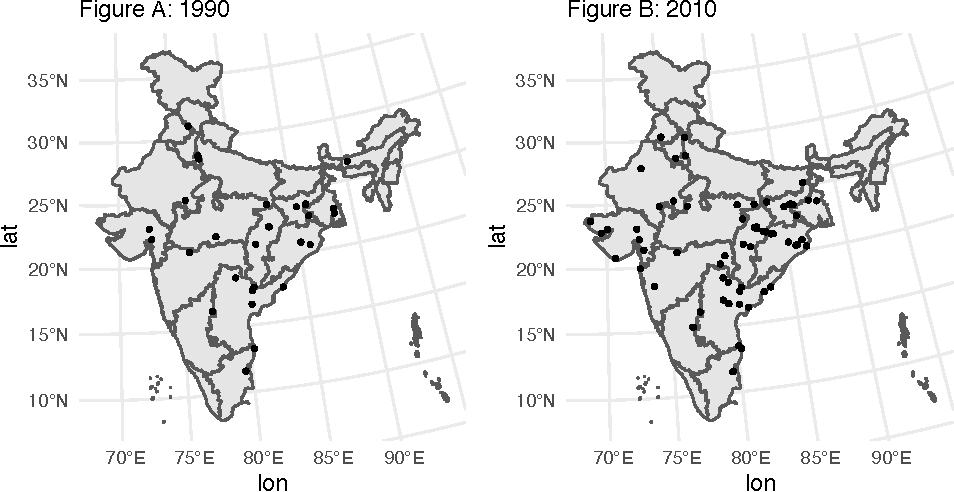
\includegraphics{draft_files/figure-latex/plants-1} \caption[Coal plants in India from 1990 to 2010]{Coal plants in India from 1990 to 2010}\label{fig:plants}\floatfoot*{Note: The top figure shows the location of coal plants in 1990. The bottom figure shows the location of coal plants in 2010.}
\end{figure}

\FloatBarrier
\newpage

\begin{figure}
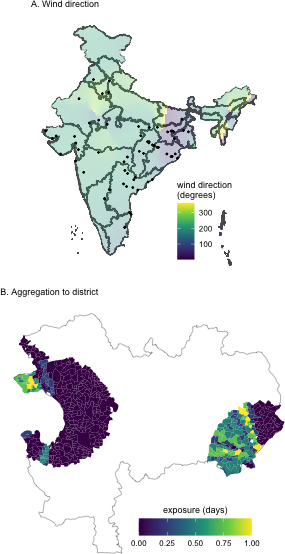
\includegraphics{draft_files/figure-latex/windexample-1} \caption[Wind direction and aggregation examples (2010-01-01)]{Wind direction and aggregation examples (2010-01-01)}\label{fig:windexample}\floatfoot*{Note: The top figure shows the average wind direction on January 1st, 2010, with zero degrees indicating north. The points are the location of coal plants on that date. The bottom figure shows the distribution of pollution exposure in a specific district -- Guna district in Madhya Pradesh -- on the same date.}
\end{figure}

\FloatBarrier
\newpage

\begin{table}

\caption{\label{tab:pollutiontable}Wind direction and particulate matter}
\centering
\begin{threeparttable}
\begin{tabular}[t]{>{\raggedright\arraybackslash}p{4cm}>{\centering\arraybackslash}p{2cm}>{\centering\arraybackslash}p{2cm}>{\centering\arraybackslash}p{2cm}>{\centering\arraybackslash}p{2cm}}
\toprule
\multicolumn{1}{c}{ } & \multicolumn{2}{c}{1998-2015} & \multicolumn{2}{c}{2002-2013} \\
\cmidrule(l{3pt}r{3pt}){2-3} \cmidrule(l{3pt}r{3pt}){4-5}
  & (1) & (2) & (3) & (4)\\
\midrule
wind (10s) & 0.0023*** & 0.0016*** & 0.0057*** & 0.0015***\\
 & (0.0005) & (0.0002) & (0.0005) & (0.0002)\\
\textbf{fixed effects:} & \textbf{} & \textbf{} & \textbf{} & \textbf{}\\
village & Yes & Yes & Yes & Yes\\
month & Yes & No & Yes & No\\
district-month & No & Yes & No & Yes\\
\midrule
observations & 24,376,458 & 24,376,458 & 16,250,973 & 16,250,973\\
\bottomrule
\end{tabular}
\begin{tablenotes}[para]
\item Note: Standard errors are in parentheses and are clustered at the village level. * p<0.10 ** p<0.05 *** p<0.01
\end{tablenotes}
\end{threeparttable}
\end{table}

\FloatBarrier
\newpage

\begin{figure}
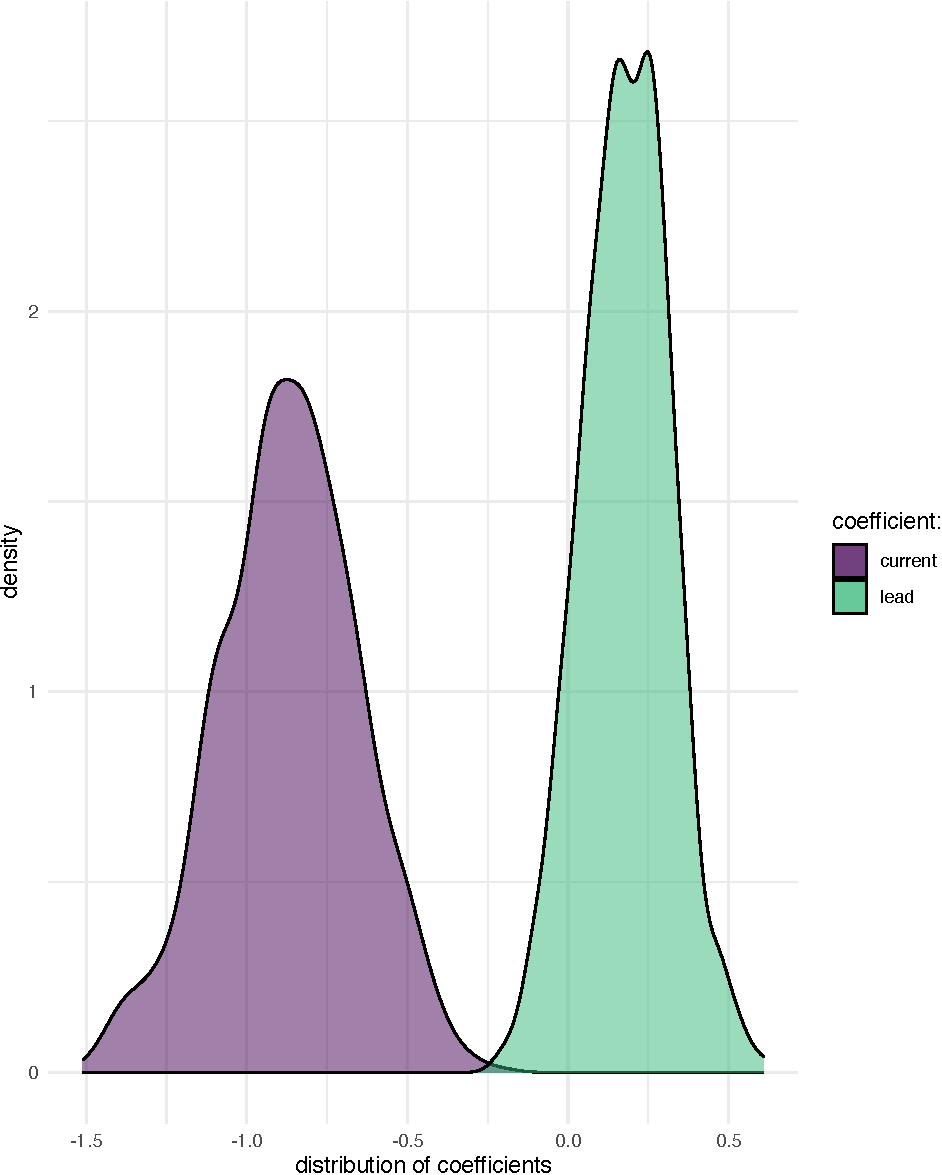
\includegraphics{draft_files/figure-latex/randomplotleads-1} \caption[Randomization inference for leads]{Randomization inference for leads}\label{fig:randomplotleads}\floatfoot*{Note: The figure presents the distribution of coefficients by randomly assigning a single wind value to each village, sampled with replacement across all villages in a given district in the same year. "Current" refers to the coefficient on current pollution, while "lead" refers to the coefficient on next year's pollution in the same table.}
\end{figure}

\FloatBarrier
\newpage

\begin{figure}
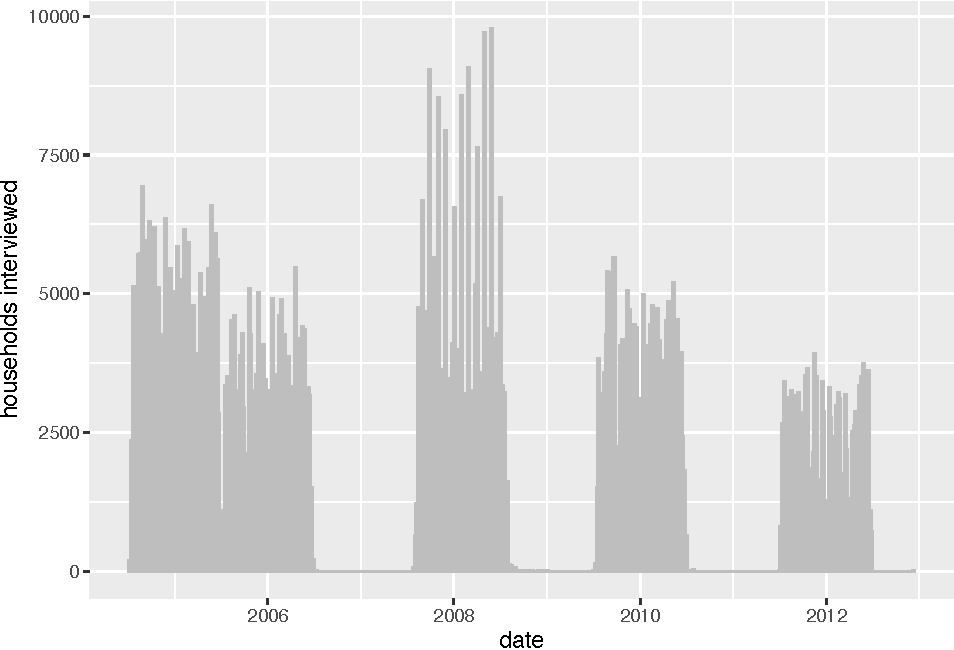
\includegraphics{draft_files/figure-latex/laborplot-1} \caption[Timing of household surveys for the National Sample Survey]{Timing of household surveys for the National Sample Survey}\label{fig:laborplot}\floatfoot*{Note: The histogram shows the distribution of survey dates for the four waves of the National Sample Survey (NSS) for the five waves used in this paper.}
\end{figure}

\FloatBarrier
\newpage

\begin{figure}
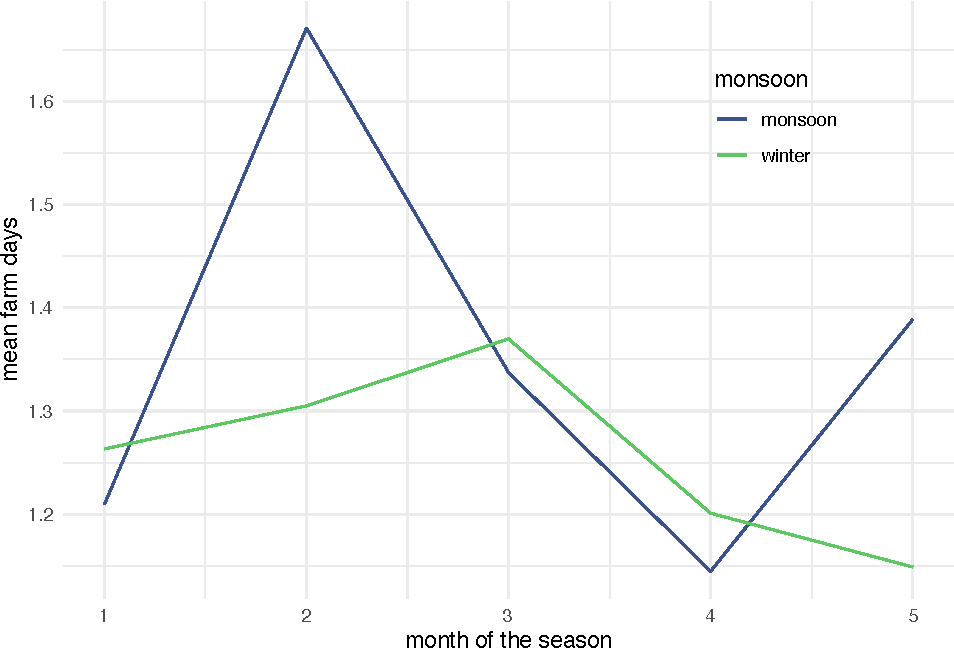
\includegraphics{draft_files/figure-latex/monthplot-1} \caption[Average farm days by season, rural only]{Average farm days by season, rural only}\label{fig:monthplot}\floatfoot*{Note: The line graph shows the mean number of farm days worked per week based on the month of the relevant agricultural season. The monsoon season is defined as June (month 1) to October (month 5) while the rainy season is defined as November (month 1) to March (month 5) of the following year. The data is from the NSS.}
\end{figure}

\FloatBarrier
\newpage

\begin{table}

\caption{\label{tab:yield8cumulative}Cumulative exposure to pollution during the season}
\centering
\begin{threeparttable}
\begin{tabular}[t]{>{\raggedright\arraybackslash}p{2.25cm}>{\centering\arraybackslash}p{2cm}>{\centering\arraybackslash}p{2cm}>{\centering\arraybackslash}p{2cm}>{\centering\arraybackslash}p{2cm}>{\centering\arraybackslash}p{2cm}}
\toprule
  & (1) & (2) & (3) & (4) & (5)\\
\midrule
June & -0.643*** &  &  &  & \\
 & (0.064) &  &  &  & \\
July &  & -0.658*** &  &  & \\
 &  & (0.045) &  &  & \\
Aug. &  &  & -0.531*** &  & \\
 &  &  & (0.049) &  & \\
Sept. &  &  &  & -0.672*** & \\
 &  &  &  & (0.047) & \\
Oct. &  &  &  &  & -0.943***\\
 &  &  &  &  & (0.069)\\
weather & Yes & Yes & Yes & Yes & Yes\\
\textbf{fixed effects:} & \textbf{} & \textbf{} & \textbf{} & \textbf{} & \textbf{}\\
village & Yes & Yes & Yes & Yes & Yes\\
year & Yes & Yes & Yes & Yes & Yes\\
\midrule
F & 1,327 & 2,830 & 2,933 & 2,413 & 1,515\\
observations & 1,266,922 & 1,266,922 & 1,266,922 & 1,266,922 & 1,266,922\\
\bottomrule
\end{tabular}
\begin{tablenotes}[para]
\item Note: Standard errors are in parentheses and are clustered at the village level. * p<0.10 ** p<0.05 *** p<0.01
\end{tablenotes}
\end{threeparttable}
\end{table}

\end{document}
